%-------------------------------
%	PACKAGES AND OTHER DOCUMENT CONFIGURATIONS
%-------------------------------

% The \vref command specifies the location of the reference

%\documentclass[
%10pt, % Main document font size
%a4paper, % Paper type, use 'letterpaper' for US Letter paper
%oneside, % One page layout (no page indentation)
%twoside, % Two page layout (page indentation for binding and different headers)
%headinclude,footinclude, % Extra spacing for the header and footer
%BCOR5mm, % Binding correction
%]{scrartcl}


\documentclass{article}


%--------------------------------------------------------------
%	REQUIRED PACKAGES
%--------------------------------------------------------------

\usepackage[
nochapters, % Turn off chapters since this is an article        
beramono, % Use the Bera Mono font for monospaced text (\texttt)
%eulermath,% Use the Euler font for mathematics
pdfspacing, % Makes use of pdftex’ letter spacing capabilities via the microtype package
dottedtoc % Dotted lines leading to the page numbers in the table of contents
]{classicthesis} % The layout is based on the Classic Thesis style



\usepackage{arsclassica} % Modifies the Classic Thesis package

\usepackage[T1]{fontenc} % Use 8-bit encoding that has 256 glyphs

\usepackage[utf8]{inputenc} % Required for including letters with accents
%--------------------------------------------------------------
% Fonts and languages
\usepackage{libertinus} % The Libertinus font
%\usepackage[adobe-utopia]{mathdesign} % The Utopia font
%\usepackage[p,osf]{scholax}
% T1 and textcomp are loaded by package. Change that here, if you want
% load sans and typewriter packages here, if needed
%\usepackage{amsmath,amsthm}% must be loaded before newtxmath
% amssymb should not be loaded
%\usepackage[scaled=1.075,ncf,vvarbb]{newtxmath}% need to scale up math package
% vvarbb selects the STIX version of blackboard bold.


\usepackage[czech]{babel} % Český jazyk
%--------------------------------------------------------------
\usepackage{graphicx} % Required for including images
\graphicspath{{Figures/}} % Set the default folder for images

\usepackage{enumitem} % Required for manipulating the whitespace between and within lists

\usepackage{lipsum} % Used for inserting dummy 'Lorem ipsum' text into the template

\usepackage{subfig} % Required for creating figures with multiple parts (subfigures)

\usepackage{amsmath,amssymb,amsthm,amsfonts} % For including math equations, theorems, symbols, etc

\usepackage{varioref} % More descriptive referencing

\usepackage[top =3 cm, bottom = 3.5 cm, left = 1.5 cm, right = 1.5 cm]{geometry}

\usepackage{mathtools}

\usepackage{float}

\usepackage{caption}

%------------------------------------------------------------
%	DIAGRAMS AND TIKZ
\usepackage{smartdiagram}
\usepackage{metalogo}
\usepackage{tikz}
\usetikzlibrary{matrix,calc}

\usepackage{hhline} % kvůli double line v tabulkách
%------------------------------------------------------------
%	THEOREM STYLES
%------------------------------------------------------------

\theoremstyle{definition} % Define theorem styles here based on the definition style (used for definitions and examples)
\newtheorem{definition}{Definice}
\newtheorem{example}{Příklad}
\newtheorem{exercise}{Cvičení}

\theoremstyle{plain} % Define theorem styles here based on the plain style (used for theorems, lemmas, propositions)
\newtheorem{theorem}{Věta}

\theoremstyle{remark} % Define theorem styles here based on the remark style (used for remarks and notes)
\newtheorem{remark}{Poznámka}



%-------------------------------------------------------------
%	HYPERLINKS
%-------------------------------------------------------------

\hypersetup{
%draft, % Uncomment to remove all links (useful for printing in black and white)
colorlinks=true, breaklinks=true, bookmarks=true,bookmarksnumbered,
urlcolor=webbrown, linkcolor=RoyalBlue, citecolor=webgreen, % Link colors
pdftitle={}, % PDF title
pdfauthor={\textcopyright}, % PDF Author
pdfsubject={}, % PDF Subject
pdfkeywords={}, % PDF Keywords
pdfcreator={pdfLaTeX}, % PDF Creator
pdfproducer={LaTeX with hyperref and ClassicThesis} % PDF producer
}

 % Include the structure.tex file which specified the document structure and layout

%----------------------------------------------------
%	MATHEMATICS
%----------------------------------------------------

% Tělesa, obory íntegrity a metrické prostory
\newcommand{\C}{\mathbb{C}}
\newcommand{\R}{\mathbb{R}}
\newcommand{\N}{\mathbb{N}}
\newcommand{\Q}{\mathbb{Q}}
\newcommand{\Z}{\mathbb{Z}}
\renewcommand{\L}[2]{L^{#1} \left( #2 \right)} % Lebesgueovy prostory

\newcommand{\vc}[1]{\boldsymbol{#1}} % vektor
\newcommand{\mat}[1]{\mathbf{#1}} % matice

\newcommand{\norm}[1]{\left \Vert #1 \right \Vert} % norma vektoru
\newcommand{\set}[1]{ \left \lbrace #1 \right \rbrace} % množina
\newcommand{\const}{\mathrm{konst}} % konstanta

\newcommand{\F}{\mathcal{F} } % Fourierova transformace
\newcommand{\La}{\mathcal{L}} % Laplaceova transformace

% Označení funkcí
\newcommand{\Res}[2]{\mathrm{Res}_{#1} \, #2 \,} % residuum
\newcommand{\sgn}{\, \mathrm{sign} \,} % signum
\newcommand{\tg}{\,\mathrm{tg}\,} % možné značení tangens


%Značení derivací a integrálů
\newcommand{\der}[2]{\frac{\mathrm{d}#1}{\mathrm{d}#2}} % obyčejná derivace
\newcommand{\pder}[2]{\frac{\partial #1}{\partial #2}} % parciální derivace
\newcommand{\tder}[3]{\left( \pder{#1}{#2} \right)_{#3 = \const}} % termodynamická derivace
\newcommand{\D}{\mathrm{d} } % integrační znamení
\newcommand{\DD}{\mathrm{D}} % absolutní derivace
\newcommand{\intR}{\int_{-\infty}^{\infty}} % integrál přes reálnou osu



% Značení posloupností, limit a sum
\newcommand{\sequence}[2]{ \left \lbrace #1 \right \rbrace_{#2=1}^\infty} % posloupnost
\newcommand{\sumnorm}[1]{\sum_{#1}^\infty} 
\newcommand{\limplus}[1]{\lim_{#1 \rightarrow + \infty}}
\newcommand{\limminus}[1]{\lim_{#1 \rightarrow - \infty}}


% VŠE záležitosti
\newcommand{\dder}[2]{\frac{\Delta #1}{\Delta #2}}


\newcommand{\arctg}{\mathrm{arctg}\,}
\newcommand{\cotg}{\mathrm{cotg}\,}
\newcommand{\arccotg}{\mathrm{arccotg}\,} % Include the mathematics.tex file which uses some mathematical operators

\hyphenation{Fortran hy-phen-ation} % Specify custom hyphenation points in words with dashes where you would like hyphenation to occur, or alternatively, don't put any dashes in a word to stop hyphenation altogether

%-------------------------------
%	TITLE AND AUTHOR(S)
%-------------------------------

%\title{\normalfont\spacedallcaps{Article Title}} % The article title

%\subtitle{Subtitle} % Uncomment to display a subtitle

\author{\spacedlowsmallcaps{Miroslav Burýšek*}} % The article author(s) - author affiliations need to be specified in the AUTHOR AFFILIATIONS block

\date{\today} % An optional date to appear under the author(s)




%-------------------------------------
%	TESTING
%-------------------------------------
% Load packages for testing
\usepackage{blindtext}
%\usepackage{showframe} % Uncomment to show boxes around the text area, margin, header and footer
%\usepackage[inline]{showlabels}  \showlabels[\small\color{JungleGreen}]{}  % Uncomment to output the content of \label commands to the document where they are used


\begin{document}

%-------------------------------------------
%	HEADERS
%-------------------------------------------

\renewcommand{\sectionmark}[1]{\markright{\spacedlowsmallcaps{#1}}} % The header for all pages (oneside) or for even pages (twoside)
%\renewcommand{\subsectionmark}[1]{\markright{\thesubsection~#1}} % Uncomment when using the twoside option - this modifies the header on odd pages
\lehead{\mbox{\llap{\small\thepage\kern1em\color{halfgray} \vline}\color{halfgray}\hspace{0.5em}\rightmark\hfil}} % The header style

\pagestyle{scrheadings} % Enable the headers specified in this block





%-----------------------------------------
%	TABLE OF CONTENTS & LISTS OF FIGURES AND TABLES
%-----------------------------------------

%\maketitle % Print the title/author/date block

\setcounter{tocdepth}{2} % Set the depth of the table of contents to show sections and subsections only

%\tableofcontents % Print the table of contents

%\listoffigures % Print the list of figures

%\listoftables % Print the list of tables






%--------------------------------------
%	ABSTRACT
%--------------------------------------

%\section*{Abstract} % This section will not appear in the table of contents due to the star (\section*)


%---------------------------------------
%	AUTHOR AFFILIATIONS
%---------------------------------------

\let\thefootnote\relax\footnotetext{\textbf{Verze:} \today }

%--------------------------------------

%\newpage % Start the article content on the second page, remove this if you have a longer abstract that goes onto the second page

%\section*{Počítání limit}

Počítat limitu z definice nebo ukazovat, že neexistuje, je náročné. Naštěstí se ukazuje, že stačí znát několik \uv{základních limit} a pro složitější posloupnosti je počítat pomocí nich. Platí totiž:
\begin{align}
    \limn (a_n \pm b_n) = \limn a_n \pm \limn b_n \:, \quad
    \limn (ca_n) = c \limn a_n \:, \quad
    \limn (a_n b_n) = \limn a_n \cdot \limn b_n \:, \quad
    \limn \frac{a_n}{b_n} = \frac{\limn a_n}{\limn b_n} \:,
\end{align}
pokud příslušné limity existují a i všechny výrazy mají smysl. Proč je důležitý poslední dovětek? Výrazy 
\begin{align}
    \infty - \infty \:,\quad 
    \frac{a}{0} \:,\quad 
    \frac{\infty}{0} \:,\quad 
    \frac{\infty}{\infty} \:.
\end{align}
definované nejsou.

\subsection*{Polynom dělený polynomem}

Nejprve se zamysleme nad limitami posloupností typu
\begin{align}
    a_n = \frac{P_k(n)}{P_l(n)} = 
    \frac{c_k n^k + c_{k-1} n^{k-1} + \cdots + c_1 n + c_0}
    {d_l n^l + d_{l-1} n^{l-1} + \cdots + d_1 n + d_0}\:,
\end{align}
kde $P_k(n)$ je nějaký polynom stupně $k$ a $P_l$ je polynom stupně $l$, $c_i$ a $d_i$ jsou nějaké koeficienty.

Zde mohou nastat tři situace:
\begin{itemize}
    \item $k<l$: jestliže polynom dole má vyšší stupeň, pak $\limn a_n = 0$.
    \item $k>l$: jestliže polynom nahoře má vyšší stupeň, pak $\limn a_n = \pm \infty$. O znaménku rozhoduje koeficient $c_k$ u nejvyššího členu.
    \item $k=l$: jestliže polynomy mají stejný stupeň, pak $\limn a_n = \frac{c_k}{d_k}$.
\end{itemize}

\begin{example}
    Spočtěme 
    \begin{align}
        \limn \frac{n^2-n}{4n^3 + 2n^2 + 1} \:.
    \end{align}
    Abychom mohli používat pravidla pro počítání limit a nedostávali nikde nedefinované výrazy, učiníme následující trik: \textbf{z čitatele i jmenovatele vytýkáme nejvyšší mocninu $n$, která se vyskytuje ve jmenovateli}. V tomto případě to je $n^3$, takže vytýkáme
    \begin{align}
        \frac{n^2-n}{4n^3 + 2n^2 + 1} = \frac{n^3 (\frac{1}{n} - \frac{1}{n^2})}{n^3 (4 + \frac{2}{n} + \frac{1}{n^3})} = \frac{\frac{1}{n} - \frac{1}{n^2}}{4 + \frac{2}{n} + \frac{1}{n^3}}\:.
    \end{align}
    Nyní už můžeme použít pravidlo o součtu a podílu limit:
    \begin{align}
        \limn \frac{\frac{1}{n} - \frac{1}{n^2}}{4 + \frac{2}{n} + \frac{1}{n^3}}
        = \frac{\limn \frac{1}{n} - \limn \frac{1}{n^2}}{\limn 4 + \limn \frac{2}{n} + \limn \frac{1}{n^3}} = \frac{0- 0}{4 + 0 + 0} = \frac{0}{4} = 0 \:.
    \end{align}
    Takže
    \begin{align}
        \limn \frac{n^2-n}{4n^3 + 2n^2 + 1} = 0\:.
    \end{align}
\end{example}

\begin{example}
    Spočtěme
    \begin{align}
        \limn \frac{n^5+ 9 n^4}{n^4 - 2n^2 + 3} \:.
    \end{align}
    Opět provedeme trik a vytkneme $n^4$:
    \begin{align}
        \limn \frac{n^5+ 9 n^4}{n^4 - 2n^2 + 3} =
        \limn \frac{n^4(n + 9)}{n^4(1 - 2 \frac{1}{n^2} + \frac{3}{n^4})} =
        \limn \frac{n + 9}{1 - 2 \frac{1}{n^2} + \frac{3}{n^4}}
        =
        \frac{\infty + 9}{1 - 0 + 0} = \infty \:.
    \end{align}
    Takže
    \begin{align}
        \limn \frac{n^5+ 9 n^4}{n^4 - 2n^2 + 3} = + \infty \:.
    \end{align}
\end{example}

\begin{example}
    Vypočítáme
    \begin{align}
        \limn \frac{1-n^4}{1+2n^3} \:.
    \end{align}

    Stejným způsobem
    \begin{align}
        \limn \frac{1-n^4}{1+2n^3} = \limn \frac{n^3(\frac{1}{n^3}-n)}{n^3(\frac{1}{n^3}+2)}
        =
        \limn \frac{\frac{1}{n^3}-n}{\frac{1}{n^3}+2}
        =
        \frac{0-\infty}{0 + 2} = - \infty \:.
    \end{align}
\end{example}

\begin{example}
    Vypočítáme
    \begin{align}
        \limn \frac{3n^4-1}{1+n+n^2-n^4} \:.
    \end{align}
    Opět provádíme stejný trik. Všimněme si, že stupeň polynomu nahoře i dole je stejný, takže výsledkem bude konečné, nenulové číslo.
    \begin{align}
        \limn \frac{3n^4-1}{1+n+n^2-n^4} =
        \limn \frac{n^4(3-\frac{1}{n^4})}{n^4(\frac{1}{n^4}+\frac{1}{n^3}+\frac{1}{n^2}-1)}
        =
        \frac{3-0}{0+0+0-1} = -3 \:.
    \end{align}
\end{example}

\begin{example}
    Spočteme
    \begin{align}
        \limn (n-n^2) \:.
    \end{align}
    Pokud bychom chtěli ihned dosadit, dostali bychom
    \begin{align}
        \limn (n-n^2) = + \infty - \infty \:,
    \end{align}
    což je nedefinovaný výraz!
    Použijeme proto opět trik, vytkneme si $n^2$:
    \begin{align}
        \limn (n-n^2) = \limn n^2 ( \frac{1}{n} - 1) = \limn n^2 \cdot \limn (\frac{1}{n}-1) = + \infty \cdot (0-1) = - \infty \:.
    \end{align}
\end{example}

\begin{example}
    Zamysleme se trochu obecněji. Vyřešme limitu 
    \begin{align}
        \limn (c_k n^k + c_{k-1} n^{k-1} + \cdots + c_1 n + c_0) \:.
    \end{align}
    Po vytknutí nejvyšší mocniny $n^k$ uvidíme, že nás zajímá pouze koeficient $c_k$ u nejvyšší mocniny, který rozhoduje o tom, zda limita bude $+\infty$ nebo $-\infty$.
    \begin{align}
        \limn (c_k n^k + c_{k-1} n^{k-1} + \cdots + c_1 n + c_0) = \limn n^k \cdot \limn (c_k + c_{k-1} \frac{1}{n} + \cdots + c_1 \frac{1}{n^{k-1}} + c_0 \frac{1}{n^k}) = +\infty \cdot c_k \:. 
    \end{align}
    Takže pokud $c_k >0$, limita bude $+\infty$, pokud $c_k<0$, bude limita $-\infty$.
\end{example}

\subsection*{Věta o dvou strážnících}

Zamysleme se nad posloupností
\begin{align}
    a_n = \frac{(-1)^n}{n^2} \:.
\end{align}
Nemůžeme použít aritmetiku limit, protože posloupnost v čitateli $(-1)^n$ limitu nemá, viz příklad výše. Přesto ale tušíme, že limita této posloupnosti bude nulová, protože do jmenovatele vstupují větší a větší čísla.

V těchto situacích se používá tvrzení, které se nazývá \textbf{věta o sevřené posloupnosti} nebo \textbf{věta o dvou strážnících} nebo též \textbf{věta o sendviči}.

Máme-li dvě posloupnosti $\set{s^{\uparrow}_n}_{n=1}^\infty$ a $\set{s^{\downarrow}_n}_{n=1}^\infty$ a posloupnosti $\set{a_n}_{n=1}^\infty$, pro které platí:
\begin{enumerate}
    \item Od jistého členu $n_0$ platí pro všechna $n>n_0$, že $s^{\downarrow}_n \leq a_n \leq s^{\uparrow}_n$,
    \item $\limn s_n^{\downarrow} = \limn s_n^{\uparrow} = A$,
\end{enumerate}
pak i \begin{align}
    \limn a_n = A \:.
\end{align}
Posloupnost $\set{s^{\uparrow}_n}_{n=1}^\infty$ funguje jako \uv{horní strážník}, posloupnost $\set{s^{\downarrow}_n}_{n=1}^\infty$ funguje jako \uv{spodní strážník}. Protože je mezi ně posloupnost $\set{a_n}_{n=1}^\infty$ \uv{vmáčknutá} a oba strážníci mají stejnou limitu, musí ji mít i $\set{a_n}_{n=1}^\infty$.

V našem příkladu můžeme najít takové dva strážníky. Horní strážník bude posloupnost
\begin{align}
    s_n^{\uparrow} = + \frac{1}{n^2}
\end{align}
a spodní strážník bude
\begin{align}
    s_n^{\downarrow} = - \frac{1}{n^2} \:.
\end{align}
Určitě platí \begin{align}
    \limn \frac{1}{n^2} = 0 = \limn -\frac{1}{n^2} \:.
\end{align}
Zároveň jistě platí, že \begin{align}
    -\frac{1}{n^2} \leq \frac{(-1)^n}{n^2} \leq +\frac{1}{n^2} \:.
\end{align}
Použijeme tedy větu o dvou strážnících a dostáváme
\begin{align}
    \limn \frac{(-1)^n}{n^2} = 0 \:.
\end{align}

\begin{example}
    Zkoumejme
    \begin{align}
        \limn \frac{\sin \left( \frac{n}{4 \pi}\right)}{n} \:.
    \end{align}
    (Cvičení: napište prvních deset členů takové posloupnosti a vyznačte je do grafu.)

    Víme, že
    \begin{align}
        -1 \leq \sin (kn) \leq +1 \quad \text{pro libovolné } k \in \R \:.
    \end{align}
    Můžeme proto najít dva strážníky. Spodní strážník bude posloupnost $s_n^{\downarrow} = -\frac{1}{n}$ a horní strážník bude $s_n^{\uparrow} = + \frac{1}{n}$. Obě dvě posloupnosti mají limitu $0$, takže
    \begin{align}
        \limn \frac{\sin \left( \frac{n}{4 \pi}\right)}{n} = 0 \:.
    \end{align}
\end{example}

\begin{example}[Malinko obtížnější]
    Zkoumejme limitu
    \begin{align}
        \limn \frac{\sin n + \cos^2 n}{n + \sin n} \:.
    \end{align}
    Opět tušíme, že díky $n$ ve jmenovateli bude limita nulová. Kvůli goniometrickým funkcím musíme opět najít dva strážníky. 
    Čitatel snadno můžeme omezit:
    \begin{align}
        -2 \leq \sin n + \cos^2 n \leq 2
    \end{align}
    a jmenovatel též:
    \begin{align}
       n-1 \leq n + \sin n \leq n + 1
    \end{align}
    Takže můžeme vzít strážníky $s_n^{\uparrow} = \frac{+2}{n - 1}$ a $s_n^{\downarrow} = \frac{-2}{n+1}$ (horní strážník je \uv{největší čitatel ku nejmenšímu jmenovateli} a spodní strážník je \uv{nejmenší čitatel ku největšímu jmenovateli}). Oba dva strážníci mají nulovou limitu, takže opět 
    \begin{align}
        \limn \frac{\sin n + \cos^2 n}{n + \sin n} = 0 \:.
    \end{align}
\end{example}


\subsection*{Limity s odmocninami}

\begin{example}
    Určíme
    \begin{align}
        \limn (n-\sqrt{n^2+4}) \:.
    \end{align}
    Cvičení: zobrazte si graf funkcí $x$ a $\sqrt{x^2+4}$. Dá se \textrm{něco} říci o chování pro $x \rightarrow +\infty$?

    Pokud bychom dosadili, dostali bychom opět $\infty - \infty$, což není definované. Musíme proto použít další trik, kterému se říká \textbf{rozšíření sdruženým výrazem}.
    Potkáme-li někde výraz typu \uv{$(\textrm{něco}) - \sqrt{\textrm{odmocnina}}$}, rozšíříme ho výrazem s opačným znaménkem \uv{$(\textrm{něco}) + \sqrt{\textrm{odmocnina}}$}. V našem případě
    \begin{align}
        n-\sqrt{n^2+4} = \left( n-\sqrt{n^2+4} \right) \cdot \frac{n + \sqrt{n^2+4}}{n + \sqrt{n^2+4}}
    \end{align}
    a podívejme se, co se stane:
    \begin{align}
        \left( n-\sqrt{n^2+4} \right) \cdot \frac{n + \sqrt{n^2+4}}{n + \sqrt{n^2+4}}
        =
        \frac{n^2 -n \sqrt{n^2+4} + n \sqrt{n^2+4} - (n^2+4)}{n + \sqrt{n^2+4}} 
        =
        \frac{n^2 - (n^2+4)}{n + \sqrt{n^2+4}} 
        =
        \frac{-4}{n + \sqrt{n^2+4}} 
        \:.
    \end{align}
    Kouzelně jsme se zbavili odmocniny v čitateli a dostali jsme konečné číslo. Ve jmenovateli nám zbyly dva výrazy, do kterých už ovšem můžeme dosadit:
    \begin{align}
        \limn \frac{-4}{n + \sqrt{n^2+4}}  =
        \frac{-4}{\infty + \infty} = 0 \:.
    \end{align}
    Takže
    \begin{align}
        \limn (n-\sqrt{n^2+4}) = 0 \:.
    \end{align}
\end{example}

\begin{example}
    \begin{align}
        \limn \frac{n^2}{\sqrt{n^4+1}} \:.
    \end{align}
    Po dosazení by nám vyšlo $\infty/\infty$, což není definované. Použijeme tedy jiný trik: vytkneme $n^2$ ve jmenovateli (do odmocniny ho převedeme jako $\sqrt{\frac{1}{n^4}}$). Pak už dostaneme konečný výraz:
    \begin{align}
        \limn \frac{n^2}{\sqrt{n^4+1}} = \limn \frac{n^2}{n^2 \cdot \sqrt{\frac{1}{n^4}}\sqrt{n^4+1}}
        =
        \limn \frac{1}{\sqrt{1 + \frac{1}{n^4}}} = 1 \:.
    \end{align}
\end{example}

\subsection*{Limity s mocninnými funkcemi}

\begin{example}
    Vypočítejme
    \begin{align}
        \limn \frac{2^n+3 \cdot 5^n}{4 - 8\cdot 2^n +3^n} \:.
    \end{align}
    Tak jako jsme u polynomů vytýkali nejvyšší mocninu ve jmenovateli, zde budeme vytýkat \textbf{mocninu s nejvyšším základem ve jmenovateli}. Zde máme $3^n$, takže vytýkáme
    \begin{align}
        \frac{2^n+3 \cdot 5^n}{4 - 8\cdot 2^n +3^n} 
        =
         \frac{
             \left( \frac{2}{3} \right)^n 
             + 3 \cdot \left(\frac{5}{3} \right)^n
             }
         {
              4 \cdot \left(\frac{1}{3} \right)^n
            - 8 \cdot \left( \frac{2}{3}\right)^n 
            + \left( \frac{3}{3} \right)^n} 
    \end{align}
    a nyní můžeme dosadit. Vzpomeňme si na geometrickou posloupnost, viz výše.
    \begin{align}
        \limn \frac{2^n+3 \cdot 5^n}{4 - 8\cdot 2^n +3^n} =
        \limn
        \frac{
            \left( \frac{2}{3} \right)^n 
            + 3 \cdot \left(\frac{5}{3} \right)^n
            }
        {
            4 \cdot \left( \frac{1}{3} \right)^n
           - 8 \cdot \left( \frac{2}{3}\right)^n 
           + \left( \frac{3}{3} \right)^n} 
        =
        \frac{0+3 \cdot \infty}{0 - 0 + 1} = + \infty \:.
    \end{align}
\end{example}

\begin{example}
    Vypočítejme
    \begin{align}
        \limn  \frac{2^n}{3 \cdot 2^n + 4}  \:.
    \end{align}
    Opět vytkneme $2^n$ a dostaneme
    \begin{align}
        \limn \frac{2^n}{3 \cdot 2^n + 4} = \limn \frac{1}{3 + \frac{4}{2^n}} = \frac{1}{3 + 0} = \frac{1}{3} \:.
    \end{align}
\end{example}

\begin{example}
    Vypočítejme (používáme zde desetinnou tečku namísto desetinné čárky)
    \begin{align}
        \limn \frac{(0.04)^{n+1}-2}{(0.2)^{2n}+4} \:.
    \end{align}
    Výpočet je jednoduchý, jen si musíme vzpomenout na pravidla pro počítání s mocninami:
    \begin{align}
        \frac{(0.04)^{n+1}-2}{(0.2)^{2n}+4} =
        \frac{0.04 \cdot (0.04)^{n} - 2}{(0.2^2)^n + 4} =
        \frac{0.04 \cdot (0.04)^{n} - 2}{(0.04)^n + 4} \:,
    \end{align}
    takže
    \begin{align}
        \limn \frac{(0.04)^{n+1}-2}{(0.2)^{2n}+4}
        =
        \limn \frac{0.04 \cdot (0.04)^{n} - 2}{(0.04)^n + 4}
        =
        \limn \frac{0 - 2}{0 +4} = - \frac{1}{2} \:.
    \end{align}
\end{example}

\subsection*{Shrnutí a závěrečné poznámky}
Typické příklady na limity posloupností spadají do jedné ze čtyř kategorií:
\begin{itemize}
    \item \textbf{Limity typu \uv{polynom/polynom}}. Zde je situace jednoduchá, vytkneme člen s nejvyšší mocninou ve jmenovateli. Mohou nastat tři situace, které se odvíjejí od stupňů jednotlivých polynomů.
    \item \textbf{Limity s mocninnými funkcemi}. Zde se vytýká mocnina s nejvyšším základem ve jmenovateli. Jinak všechno stojí na pochopení geometrické posloupnosti.
    \item \textbf{Limity s periodickými funkcemi a $(-1)^n$}. Zde se používá věta o dvou strážnících. Důležité je nalézt správně horního a spodního strážníka.
    \item \textbf{Limity s odmocninou}. Zde se vyplatí většinou rozšiřovat sdruženým výrazem. Vyžadují asi nejvíce cviku.
\end{itemize}

Později se seznámíme s tzv. l'Hospitalovým pravidlem, které nám umožní počítat některé limity daleko rychleji. Vyžaduje ale umění derivací. 

%\section*{Počítání limit funkcí}

Aritmetika limit platí i pro funkce. Typově se používají podobné triky jako v příkladech pro limity posloupností. Základní limity jsou uvedeny zde:

\begin{align}
    &\lim_{x \rightarrow - \infty } \frac{1}{x} = 0 = \lim_{x \rightarrow + \infty } \frac{1}{x} \:, \quad
    \lim_{x \rightarrow 0-} \frac{1}{x} = - \infty \:, \quad \lim_{x \rightarrow 0+} \frac{1}{x} = + \infty \:, \\
    &\lim_{x \rightarrow + \infty} x^k = + \infty \text{ pro jakékoli } k \in \N \:, \quad
    \lim_{x \rightarrow - \infty} x^k = \begin{cases}
        + \infty & \text{ pro } k \text{ sudé} \\
        - \infty & \text{ pro } k \text{ liché}
    \end{cases} \:, \\
    &\lim_{x \rightarrow +\infty} e^x = + \infty \:, \quad \lim_{x \rightarrow -\infty} e^x = 0 \:, \\
    &\lim_{x \rightarrow 0+} \ln x = - \infty \:, \quad \lim_{x \rightarrow +\infty} \ln x = + \infty \:,\\
    &\lim_{x \rightarrow \pm \infty} \sin x \:, \quad \lim_{x \rightarrow \pm \infty} \cos x  \text{ neexistují} \:, \\
    &\lim_{x \rightarrow -\infty} \arctg x = - \frac{\pi}{2} \:, \quad \lim_{x \rightarrow +\infty} \arctg x = \frac{\pi}{2} \:, \\
    &\lim_{x \rightarrow -\infty} \arccotg x = \pi \:, \quad \lim_{x \rightarrow +\infty} \arccotg x = 0 \:.
\end{align}


\begin{example}
    Spočteme
    \begin{align}
        \lim_{x \rightarrow -\infty} \frac{2x^3-4x^2+x+1}{x^2-8x} \:.
    \end{align}
    Pokud počítáme nevlastní limitu podílu polynomů, využíváme triku vytýkání nejvyšší mocniny ve jmenovateli. Takže vytkneme $x^2$ a máme
    \begin{align}
        \lim_{x \rightarrow -\infty} \frac{2x^3-4x^2+x+1}{x^2-8x} =
        \lim_{x \rightarrow -\infty} \frac{x^2 \left( 2x - 4 + \frac{1}{x} + \frac{1}{x^2}\right)}{x^2 \left( 1 - \frac{8}{x} \right)} =
        \lim_{x \rightarrow -\infty} \frac{2x - 4 + \frac{1}{x} + \frac{1}{x^2}}{1 - \frac{8}{x}}
    \end{align}
    a do takového výrazu již můžeme dosadit. Jenom opatrně, dosazujeme $-\infty$, takže
    \begin{align}
        \lim_{x \rightarrow -\infty} \frac{2x^3-4x^2+x+1}{x^2-8x} = \frac{2 \cdot (-\infty) - 4 + 0 + 0}{1 - 0} = - \infty \:.
    \end{align}
\end{example}


\subsection*{Limity typu \uv{$\frac{a}{0}$}.}

Již víme, že $\frac{a}{0}$ není definovaný výraz. Nyní se musíme naučit vypořádat s limitami podílu polynomů ve vlastních bodech, kde se takové výrazy objeví. Využijeme k tomu následující tvrzení.

Jestliže platí
\begin{align}
    \lim_{x \rightarrow x_0+} f(x) = 0 \:, \quad f(x) \geq 0 \text{ na pravém okolí } P^+(x_0) \:,
\end{align}
pak
\begin{align}
    \lim_{x \rightarrow x_0+} \frac{1}{f(x)} = + \infty \:.
\end{align}
Jestliže platí
\begin{align}
    \lim_{x \rightarrow x_0+} f(x) = 0 \:, \quad f(x) \leq 0 \text{ na pravém okolí } P^+(x_0) \:,
\end{align}
pak
\begin{align}
    \lim_{x \rightarrow x_0+} \frac{1}{f(x)} = - \infty \:.
\end{align}
Analogické tvrzení platí pro limitu zleva a levé okolí.

\begin{example}
    Vypočítejme limity \begin{align}
        \lim_{x \rightarrow 2-} \frac{1}{x-2} \:, \quad \lim_{x \rightarrow 2+} \frac{1}{x-2} \:, \quad \lim_{x \rightarrow 2} \frac{1}{x-2} \:.
    \end{align}
    Platí $\lim_{x \rightarrow 2-} (x-2) = 0 = \lim_{x \rightarrow 2+} (x-2) \:.$
    Nyní se stačí podívat na to, jaké znaménko má funkce $(x-2)$ na levém a pravém okolí dvojky.
    \begin{itemize}
        \item Na levém okolí nuly, tj. pro $x<2$, je $x-2<0$. Proto podle předchozího tvrzení platí \begin{align}
            \lim_{x \rightarrow 2-} \frac{1}{x-2} = - \infty \:.
        \end{align}

        \item Na pravém okolí nuly, tj. pro $x>2$, je $x-2>0$. Proto podle předchozího tvrzení platí \begin{align}
            \lim_{x \rightarrow 2-} \frac{1}{x-2} = + \infty \:.
        \end{align}

        \item Protože se limita zprava a zleva nerovnají,
        \begin{align}
            \lim_{x \rightarrow 2} \frac{1}{x-2} \text{ neexistuje} \:. 
        \end{align}
    \end{itemize}

\end{example}


\begin{example}
    Nechť \begin{align}
        f(x) = \frac{x^3-2x^2+1}{x^2-4} \:.
    \end{align}
    Vypočteme
    \begin{enumerate}[label=(\roman*)]
        \item $\lim_{x \rightarrow +\infty} f(x)$,
        \item $\lim_{x \rightarrow -\infty} f(x)$,
        \item $\lim_{x \rightarrow 0} f(x)$,
        \item $\lim_{x \rightarrow -2 -} f(x)$,
        \item $\lim_{x \rightarrow -2 +} f(x)$,
        \item $\lim_{x \rightarrow 2 -} f(x)$,
        \item $\lim_{x \rightarrow -2 +} f(x)$.
    \end{enumerate}

    \begin{enumerate}[label=(\roman*)]
        \item Zde nemůžeme dostadit přímo, dostali bychom $\frac{\infty}{\infty}$. Můžeme si ale pomoci stejným trikem jakou u posloupností: \begin{align}
            \lim_{x \rightarrow +\infty} \frac{x^3-2x^2+1}{x^2-4} =
            \lim_{x \rightarrow +\infty} \frac{x - 2 + \frac{1}{x^2}}{1 - \frac{4}{x^2}} =
            \frac{+\infty - 2 + 0}{1 - 0} = + \infty \:.
        \end{align}

        \item \begin{align}
            \lim_{x \rightarrow -\infty} \frac{x^3-2x^2+1}{x^2-4} =
            \lim_{x \rightarrow -\infty} \frac{x - 2 + \frac{1}{x^2}}{1 - \frac{4}{x^2}} =
            \frac{-\infty - 2 + 0}{1 - 0} = - \infty \:.
        \end{align}

        \item Zde dosadit můžeme rovnou, nedostaneme se k nedefinovanému výrazu: \begin{align}
            \lim_{x \rightarrow 0} \frac{x^3-2x^2+1}{x^2-4} =
            \frac{0-0+1}{0-4} = - \frac{1}{4} \:.
        \end{align}

        \item Kdybychom dosadili rovnou, dostali bychom
        \begin{align}
            \lim_{x \rightarrow -2 -} \frac{x^3-2x^2+1}{x^2-4} = \frac{-8 - 8 + 1}{4 - 4} = \frac{-15}{0} \:,
        \end{align}
        což není definovaný výraz. Proto máme co do činění s limitou typu $\frac{a}{0}$. V tom případě se podíváme na to, jaké znaménko má funkce ve jmenovateli na levém okolí minus dvojky: $x^2-4 > 0$ pro $x<-2$. Takže 
        \begin{align}
            \lim_{x \rightarrow -2 -} \frac{1}{x^2-4} = - \infty \:.
        \end{align}
        Nyní už stačí použít aritmetiku limit (čitatel má limitu konečnou):
        \begin{align}
            \lim_{x \rightarrow -2 -} \frac{x^3-2x^2+1}{x^2-4} = \lim_{x \rightarrow -2 -} (x^3-2x^2+1) \cdot \lim_{x \rightarrow -2 -} \frac{1}{x^2-4} = -15 \cdot (-\infty) = + \infty \:.
        \end{align}

        \item Podobně, $x^2-4<0$ pro $-2<x<2$, takže na pravém okolí $-2$ je jmenovatel záporný. Proto
        \begin{align}
            \lim_{x \rightarrow -2 +} \frac{x^3-2x^2+1}{x^2-4} = \lim_{x \rightarrow -2 +} (x^3-2x^2+1) \cdot \lim_{x \rightarrow -2 +} \frac{1}{x^2-4} = -15 \cdot (+\infty) = - \infty \:.
        \end{align}
        \item Analogicky.
        \item Analogicky.
    \end{enumerate}
\end{example}

\begin{example}
    Určíme limitu
    \begin{align}
        \lim_{x \rightarrow 3+} \frac{x^2}{6-2x} \:.
    \end{align}
    Opět vidíme
    \begin{align}
        \lim_{x \rightarrow 3+} 6 - 2x = 0 \:, \quad 6 - 2x < 0 \text{ pro } x>3 \:,
    \end{align}
    tedy podle tvrzení o $\frac{a}{0}$ platí
    \begin{align}
        \lim_{x \rightarrow 3+} \frac{x^2}{6-2x} = 9 \cdot (+\infty) = + \infty \:.
    \end{align}
\end{example}

\begin{example}
    Určíme limitu
    \begin{align}
        \lim_{x \rightarrow 1-} \frac{x^2-2x+1}{x^3-x} \:.
    \end{align}
    Pokud bychom použili tvrzení $\frac{a}{0}$ hned, dostali bychom nedefinovaný výraz
    \begin{align}
        \lim_{x \rightarrow 1-} \frac{x^2-2x+1}{x^3-x} = \lim_{x \rightarrow 1-} (x^2-2x+1) \cdot \lim_{x \rightarrow 1-} \frac{1}{x^3-x} = 0 \cdot \infty \:.
    \end{align}
    To se stalo díky tomu, že čitatel má kořen roven $1$. Stačí ho tedy rozložit do závorek a něco zkrátit:
    \begin{align}
        \lim_{x \rightarrow 1-} \frac{x^2-2x+1}{x^3-x} = \lim_{x \rightarrow 1-} \frac{(x-1)^2}{x(x-1)(x+1)} = \lim_{x \rightarrow 1-} \frac{x-1}{x(x+1)}
    \end{align}
    a můžeme klidně dosadit
    \begin{align}
        \lim_{x \rightarrow 1-} \frac{x-1}{x(x+1)} = \frac{0}{2} = 0 \:.
    \end{align}
\end{example}



%\section*{Domácí úkol 4}
\textbf{Termín odevzdání:} na cvičení 11. nebo 12.11.2021.
\newline
\textbf{Zadání:} Cílem tohoto úkolu je pořádně procvičit počítání limit posloupností a funkcí.

\begin{itemize}
    \item \textbf{(0.5 bodu)} Vymyslete tři příklady limit typu
    \begin{align}
        \lim_{n \rightarrow \infty} \frac{P_k(n)}{P_l(n)} = \lim_{n \rightarrow \infty} \frac{\text{polynom stupně }k}{\text{polynom stupně }l} \:; \quad k,l \geq 5
    \end{align}
    tak, aby hodnota limity byla
    \begin{enumerate}
        \item $-\infty$,
        \item $2021$,
        \item $0$.
    \end{enumerate}
    Výpočtem ověřte.

    \item \textbf{(0.5 bodu)} Vymyslete tři příklady limit typu
    \begin{align}
        \lim_{x \rightarrow x_0+} \frac{P_k(x)}{P_l(x)} = \lim_{x \rightarrow x_0+} \frac{\text{polynom stupně }k}{\text{polynom stupně }l} \:; \quad k,l \geq 5 \:, x_0 \text{ je vlastní bod}
    \end{align}
    tak, aby hodnota limity byla
    \begin{enumerate}
        \item $+\infty$,
        \item $0$,
        \item $1$.
    \end{enumerate}

    \item \textbf{(0.5 bodu)} Vymyslete příklad limity funkce, při jejímž výpočtu použijete větu o dvou strážnících. \textbf{NEBO:} Vymyslete příklad limity složené funkce, která obsahuje funkci $\ln x$ jako vnější funkci a její limitní hodnota bude $0$.
    
    \item \textbf{(0.5 bodu)} Vymyslete příklad limity funkce typu
    \begin{align}
        \lim_{x \rightarrow \infty} \ln f(x) \cdot \arctg g(x) \:,
    \end{align}
    kde zvolíte funkce $f(x)$ a $g(x)$ vhodně tak, aby hodnota limity byla $-\frac{\pi}{2}$.
\end{itemize}

\section*{Derivace funkce}

Derivace funkce v bodě umožňuje popsat, jak rychle se funkce v takovém bodě funkce mění.

\subsection*{Lineární funkce}

Lineární funkce jsou funkce tvaru $y(x) = ax+b$, kde $a$ a $b$ jsou určité koeficienty. Víme, že grafem lineární funkce je přímka a také, jaký vliv na ni mají $a$ a $b$:
\begin{itemize}
    \item Koeficient $b$ je tzv. \textbf{absolutní koeficient}. Udává hodnotu funkce v bodě nula. Čím je $b$ větší, tím více posouvá graf funkce $y(x)$ nahoru.
    \item Koeficient $a$ je tzv. \textbf{lineární koeficient} neboli \textbf{směrnice} přímky. Udává sklon přímky. Čím je $a$ větší, tím je graf funkce strmější. Pro $a>0$ je funkce rostoucí, pro $a=0$ přejde funkce na obyčejnou konsatntní funkci $y=b$ s nulovým sklonem, pro $a<0$ je funkce klesající.
\end{itemize}

Uvažujme nyní lineární funkce $y(x)=ax+b$ a nějaký pevný bod $x_0$ s funkční hodnotou $y(x_0)$. Ptejme se nyní, co se stane, zvětšíme-li hodnotu $x$ o nějakou vzdálenost $\D x$. Jak se změní funkční hodnota? Nakreslíme-li si situaci, vidíme, že se hodnota změní o $\D y = \D x \cdot a$. Můžeme tedy zapsat
\begin{align}
    a = \frac{\D y}{\D x} \:.
\end{align}
Představme si třeba funkci $y(x)=2x+4$ a bod $x_0=2$. Posuneme-li se o $\D x = 1$, pak se změní hodnota $y$ o $\D y = a \cdot \D x = 2 \cdot 1 = 2$. Posuneme-li se o $\D x = 2$, změní se hodnota $y$ o $\D y = 2 \cdot 2 = 4$, atd\dots

\begin{figure}[H]
    \centering
    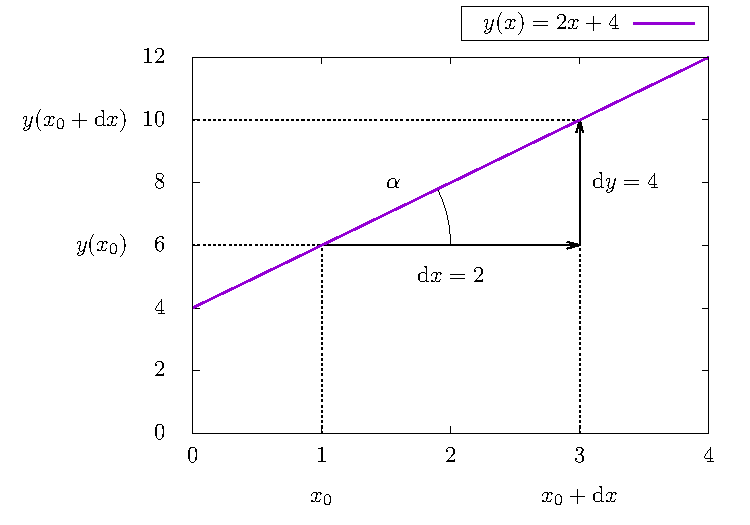
\includegraphics{Gnuplot/cv8/Figures/primka-graf.pdf}
    \caption{Znázorněna funkce $y(x)=2x+4$. Zafixujme bod $x_0=2$ s hodnotou $y(x_0)=6$. Pokud se změní $x$ o hodnotu $\D x = 2$, změní se hodnota $y$ o $\D y = \D x \cdot 2 = 4$.}
\end{figure}

To, že při posunu o $\D x$ snadno spočteme $\D y$ pouhým vynásobení číslem, je vlastnost, která platí pouze pro lineární funkce. Proto jsou vlastně lineární funkce tak speciální. U složitějších funkcí už obecně záleží na tom, jak velké je $x$ a $\D x$. Uvažte například kvadratickou funkci, tam už přírůstek $\D y$ bude pokaždé jiný.

\subsection*{Derivace jako tečna funkce}

Pakliže však bude funkce \uv{dostatečně rozumná} a ono $\D x$ dostatečně malé, máme návod na to, jak určit malou změnu v $\D y$. Můžeme se totiž na nějakém malém okolí bodu $x_0$ pokusit aproximovat funkci její \textbf{tečnou}. Jak vytvořit tečnu ke křivce v daném bodě? Začneme tím, že vytvoříme \textbf{sečnu}, přímku spojující dva body na grafu funkce. Jeden bod bude $(x_0,f(x_0))$. Druhý bod vezměme tak, že posuneme bod $x_0$ o nějakou vzdálenost $h$ a získáme bod $(x_0+h,f(x_0+h))$.

\begin{figure}[H]
    \centering
    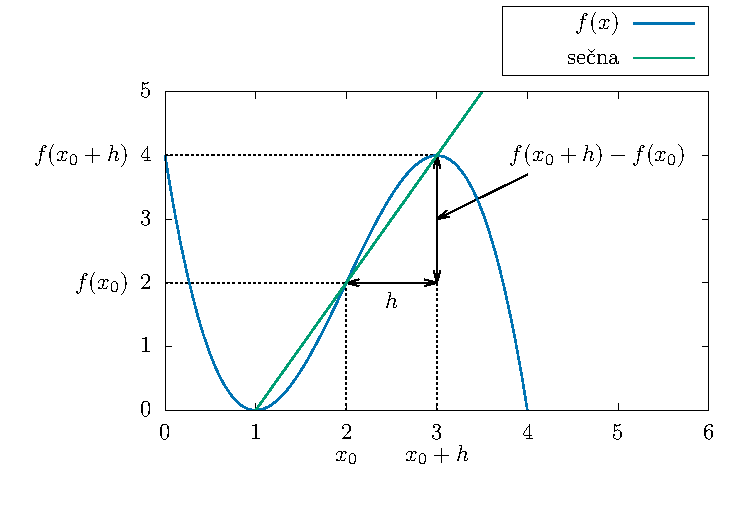
\includegraphics{Gnuplot/cv8/Figures/secna-graf.pdf}
    \caption{Příklad konstrukce sečny k nějaké funkci (modrá). Vezmeme bod $x_0=2$ s funkční hodnotou $f(x_0)=2$. Druhý bod vezmeme tak, že k $x_0$ přičteme $h=1$. Odpovídající funkční hodnota je $f(x_0+h)=4$. Takto získané body propojíme přímkou (zelená).}
\end{figure}

Nyní si všimneme, že čím blíže bude druhý bod prvnímu, tím lépe se sečna podobá tečně. Pokud budeme zmenšovat onu vzdálenost $h$ mezi dvěma body (přičemž $x_0$ ponecháváme stále na místě), bude se směrnice sečen stále více přibližovat směrnici tečny.

\begin{figure}[H]
    \centering
    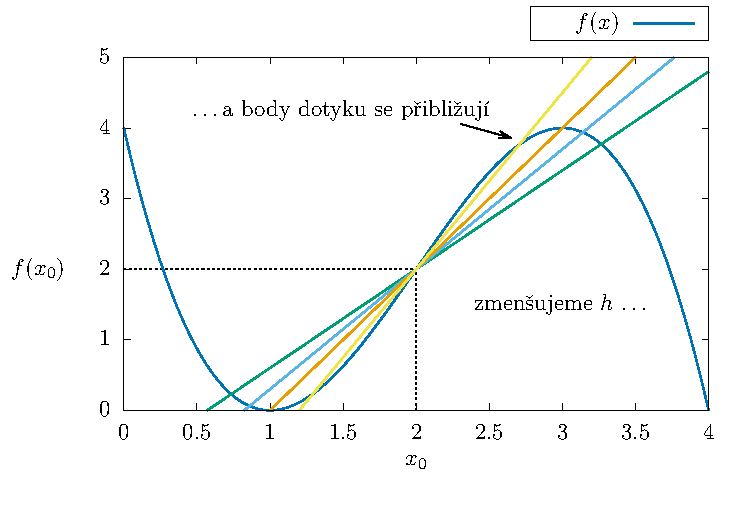
\includegraphics{Gnuplot/cv8/Figures/priblizovani-graf.pdf}
\end{figure}

Až nakonec pro $h \rightarrow 0$ přejdou sečny skutečně v tečnu.

\begin{figure}[H]
    \centering
    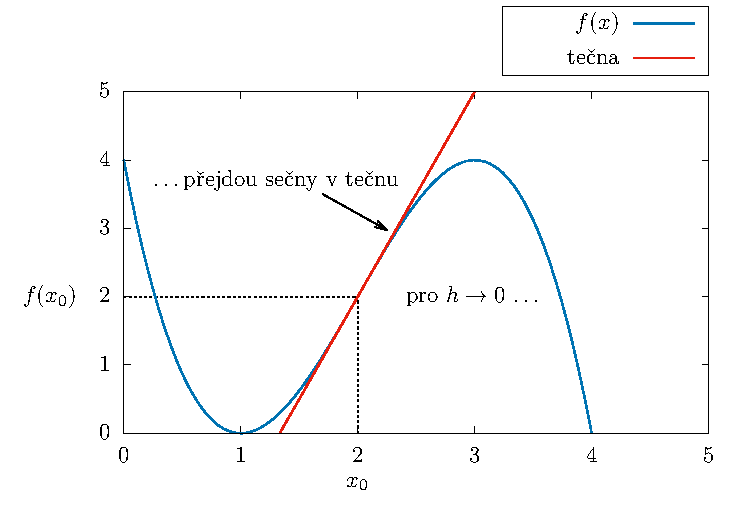
\includegraphics{Gnuplot/cv8/Figures/tecna-graf.pdf}
\end{figure}

Pokud nyní vezmeme $\D x$ dostatečně malé, nebude nám vadit, když místo skutečné hodnoty $\D y$ budeme počítat s přibližnou hodnotou, kterou nám bude dávat bod na tečně.

Vraťme se k předchozímu obrázku. Jaká je směrnice zelené sečny? Je to zase podíl toho, o kolik se změnila funkční hodnota, a toho, o kolik jsme se posunuli:
\begin{align}
    \text{směrnice sečny} = \frac{\text{o kolik se změní funkce}}{\text{o kolik se posuneme}} = \frac{f(x_0+h)-f(x_0)}{(x_0+h)-x_0} = \frac{f(x_0+h)-f(x_0)}{h} \:.
\end{align}
Směrnici tečny získáme limitním procesem
\begin{align}
    \text{směrnice tečny} = \lim_{h \rightarrow 0} \text{směrnice sečny} = \lim_{h \rightarrow 0} \frac{f(x_0+h)-f(x_0)}{h} \:.
\end{align}
Získáváme tak vztah pro \textbf{derivaci funkce $f$ v bodě} $x_0$:
\begin{align}
    \boxed{\frac{\D f}{\D x} (x_0) = f'(x_0) = \lim_{h \rightarrow 0} \frac{f(x_0+h)-f(x_0)}{h}} \:.
\end{align}
Ještě jednou, derivace funkce $f$ v bodě $x_0$ představuje směrnici tečny k takové funkci v bodě $x_0$. K čemu je to dobré? Pokud se posuneme o nějaké $\D x$ a ptáme se, o jakou hodnotu $\D f$ se funkce $f$ změní, můžeme použít jednoduchý vztah:
\begin{align}
    \D f = \D x \cdot f'(x_0) \:.
\end{align}
Dokonce si můžeme napsat celý předpis pro tečnu:
\begin{align}
    \text{rovnice tečny} = y(x) = f'(x_0) \cdot (x-x_0) + f(x_0) \:.
\end{align}
Přírůstek $x-x_0$ je právě posunutí mezi $x_0$ a $x$. Zajímá-li nás hodnota tečny v bodě $x$, stačí takové posunutí vynásobit derivací funkce $f'(x_0)$ a přičíst ještě funkční hodnotu $f(x_0)$.

\subsection*{Jak derivaci počítat?}

Můžeme ji počítat přímo z definice.

\begin{example}[Derivace lineární funkce]
    Výše jsme uvedli, že lineární funkce $y(x)=ax+b$ má všude stále stejnou směrnici $a$. To znamená, že lineární funkce splývá se svou tečnou a derivace by měla být rovna směrnici $a$. To se dá samozřejmě ukázat i matematicky:
    \begin{align}
        y'(x_0) = \lim_{h \rightarrow 0} \frac{y(x_0+h)-y(x_0)}{h} = \lim_{h \rightarrow 0} \frac{[a(x_0+h)+b]-[a x_0 + b]}{h} = 
        \lim_{h \rightarrow 0} \frac{ah}{h} = \lim_{h \rightarrow 0} a = a \:. 
    \end{align}
    Vidíme, že derivace je všude rovna $a$, nezávisle na tom, v jakém bodě $x_0$ ji počítáme.
\end{example}

\begin{example}[Kvadratická funkce]
    Jak to bude u kvadratické funkce $f(x)=x^2$? Čekáme, že zde již derivace bude záviset na bodě $x_0$, kde ji počítáme. Parabola se totiž stává stále strmější a strmější. Výpočet dává
    \begin{align}
        f'(x_0) = \lim_{h \rightarrow 0} \frac{[(x_0+h)^2]-[x_0^2]}{h} = 
        \lim_{h \rightarrow 0} \frac{2 x_0 h + a h^2 }{h} =
        \lim_{h \rightarrow 0} (2 x_0 + ah) = 2 x_0 \:.
    \end{align}
    Derivace je tedy různá v každém bodě $x_0$. Čím větší je bod $x_0$, tím větší je derivace. To přesně odpovídá tomu, že je ve vzdálenějších bodech parabola strmější a strmější.
\end{example}

\begin{example}[Nepřímá úměrnost]
    Jaká bude derivace u funkce $g(x)=\frac{1}{x}$? Čekáme, že derivace určitě záporná, neboť nepřímá úměrnost je klesající, tečna bude tedy taky klesající. Navíc čím větší bude $x_0$, tím se pokles funkce zpomaluje. Výpočtem ukážeme
    \begin{align}
        g'(x_0) = \lim_{h \rightarrow 0} \frac{\frac{1}{x_0+h}-\frac{1}{x_0}}{h} =
        \lim_{h \rightarrow 0} \frac{1}{h} \frac{(x_0)-(x_0+h)}{(x_0+h)x_0} = 
        \lim_{h \rightarrow 0} \frac{-h}{h (x_0+h) x_0} = 
        \lim_{h \rightarrow 0} \frac{-1}{(x_0+h) x_0} = -\frac{1}{x_0^2} \:.
    \end{align}
    To je přesně to, co jsme čekali.
\end{example}

Počítání z definice je ale poměrně zdlouhavé, jakmile jsou předpisy pro funkce složitější. Naštěstí platí stejná pravidla pro aritmetiku derivací, jako pro aritmetiku limit.

\section*{Počítání derivací}

Derivace elementárních funkcí je potřeba naučit se nazpaměť z tabulky.

\subsection*{Derivace polynomů a obecné mocniny}

Pro derivaci mocniny se používá vztah
\begin{align}
    (x^k) = k x^{k-1} \quad \text{platný pro } k \in \R \:.
\end{align}
Všimněme si, že se výpočet sestává ze dvou kroků. Mocnina $k$ u $x^k$ \uv{spadne} před něj a v exponentu zůstane mocnina o jedničku snížená, $x^{k-1}$, dohromady $k x^{k-1}$.

\begin{example}
    Spočítáme derivaci funkce 
    \begin{align}
        f(x) = 2x^3 - 4x^2 + 8x - 1 \:.
    \end{align}

    Můžeme derivovat člen po členu: 
    \begin{align}
        (2x^3)'=2 \cdot (x^3)' = 2 \cdot (3 x^2) = 6 x^2 \:.
    \end{align}
    Obdobně
    \begin{align}
        (4x^2)' = 4 \cdot 2x = 8x \:.
    \end{align}
    Připomeňme, že $x^1=x$ a $x^0=1$. Z třetího členu dostaneme tedy
    \begin{align}
        (8x)'=(8x^1)'=8 \cdot (1x^0)= 8 \cdot (1 \cdot 1) = 8
    \end{align}
    a ze čtvrtého
    \begin{align}
        (1)' = 1 \cdot (x^0)'= 1 \cdot (0 \cdot x^{-1}) = 0 \:. 
    \end{align}
    Teď stačí jen všechno sečíst:
    \begin{align}
        f'(x) =  6 x^2 - 8x + 8 \:.
    \end{align}
\end{example}

\begin{example}
    Spočítáme derivaci funkce
    \begin{align}
        g(x) = x^{10} + \frac{1}{x^{10}} \:.
    \end{align}
    Na první člen použijeme vztah a máme $(x^{10})' = 10 x^9$. Druhý člen $\frac{1}{x^{10}}$ se dá stejně tak zapsat jako $x^{-10}$ a platí pro něj stejné pravidlo:
    \begin{align}
        \left( \frac{1}{x^{10}}\right)' = (x^{-10})' = (-10) x^{-11} = - \frac{10}{x^{11}} \:.
    \end{align}
    Pozor, často má člověk tendenci dělat v tomto chyby a psát $(x^{-10})'=-10 x^{-9}$, což je chyba!
    Celkově 
    \begin{align}
        g'(x) = 10 x^9 - \frac{10}{x^{11}} \:.
    \end{align}
\end{example}

\subsection*{Derivace ostatních elementárních funkcí}

\begin{example}
    Spočteme
    \begin{align}
        (\sin x - \cos x)' \:.
    \end{align}

    Platí
    \begin{align}
        (\sin x - \cos x)' = (\sin x)' - (\cos x)' = \cos x + \sin x \:.
    \end{align}
\end{example}

\begin{example}
    \begin{align}
        [4e^{3x} + \ln (4x) - \arctg x]' =& 4 (e^{3x})' + (\ln 4 + \ln x)' - (\arctg x)' = 4 \cdot 3 e^{3x} + 0 + \frac{1}{x} - \frac{1}{1+x^2} = \\
        =& 12 e^{3x} + \frac{1}{x} - \frac{1}{1+x^2} \:.
        \:.
    \end{align}
\end{example}

\subsection*{Derivace součinu a podílu}

Pro derivaci součinu platí
\begin{align}
    (fg)'=f'g + f g' \neq f'g'
\end{align}
a pro derivaci podílu platí
\begin{align}
    \left( \frac{f}{g} \right)' = \frac{f'g - g' f}{g^2} \neq \left( \frac{f'}{g'} \right) \:.
\end{align}

\begin{example}
    \begin{align}
        \left[ (2x+4)\cdot x^4 \right]' = (2x+4)' x^4 + (2x+4) (x^4)' = 2 x^4 + 
        (2x+4) \cdot 4x^3 = 2 x^4 + 8x^4 + 16 x^3 = 10 x^4 + 16 x^3 \:.
    \end{align}
\end{example}

\begin{example}
    \begin{align}
        (x \sin x)' = \sin x + x \cos x \:.
    \end{align}
\end{example}

\begin{example}
    Pravidlo platí i pro více součinů:
    \begin{align}
        (fgh)' = f'gh+fg'h+fgh' \:.
    \end{align}
    Například
    \begin{align}
        [(x^2+4x+1)(x-2)e^{2x}]' =& \textcolor{blue}{(x^2+4x+1)'}(x-2)e^{2x} + (x^2+4x+1)\textcolor{blue}{(x-2)'}e^{2x} + (x^2+4x+1)(x-2) \textcolor{blue}{(e^{2x})'} = \\
        =& (2x + 4)(x-2)e^{2x} + (x^2+4x+1) \cdot 1 \cdot e^{2x} + (x^2+4x+1)(x-2) \cdot 2e^{2x} = \\
        =& (2x^2+4x-4x-8) e^{2x} + (x^2+4x+1) e^{2x} + (2x^3+8x^2-2x-4x^2-16x-4)e^x = \\
        =& (2x^3 + 7x^2 - 14x - 11) e^x \:.
    \end{align}
\end{example}

\begin{example}
    \begin{align}
        (\arcsin x \sin x)' = \frac{1}{\sqrt{1-x^2}} \sin x + \arcsin x \cos x \:. 
    \end{align}
\end{example}

\begin{example}
    \begin{align}
        \left( \frac{x^2+7x}{x^2-1} \right)' =& \frac{(x^2-1)(x^2+7x)'-(x^2-1)'(x^2+7x)}{(x^2-1)^2} = 
        \frac{(x^2-1)(2x+7)-(2x)(x^2+7x)}{(x^2-1)^2} = \\
        =&
        \frac{2x^3 - 2x + 7x^2 - 7 - 2x^3 - 14 x^2}{(x^2-1)^2} =
        \frac{-7x^2 - 2x - 7}{x^4 - 2x^2 + 1} \:.
    \end{align}
\end{example}

\begin{example}
    Pokud člověk zapomene vztah pro derivaci funkce $\tg x$, není problém si ji spočítat:
    \begin{align}
        (\tg x)' = \left( \frac{\sin x}{\cos x} \right)' = \frac{(\sin x)' \cos x - (\cos x)' \sin x}{\cos^2 x} = \frac{\cos^2 x + \sin^2 x}{\cos^2 x}\:.
    \end{align}
    Poslední člen lze upravit dvěma způsoby. Buďto jako součet zlomků
    \begin{align}
        (\tg x)' = \frac{\cos^2 x + \sin^2 x}{\cos^2 x} = 1 + \tg^2 x 
    \end{align}
    anebo s využitím identity $\sin^2 x + \cos^2 x = 1$,
    \begin{align}
        (\tg x)' = \frac{\cos^2 x + \sin^2 x}{\cos^2 x} = \frac{1}{\cos^2 x} \:.
    \end{align}
\end{example}

\end{document}